%% -*- coding: utf-8; -*-
% Use a opção 'digital' para ativar o retorno de referências. Essa função é indicada para a versão digital do documento
%\documentclass[phd,american]{thesispuc}%english thesis
%\documentclass[mscr,american]{thesispuc}%english dissertation
\documentclass[phd,brazilian,digital]{thesispuc}%tese em portugês
%\documentclass[msc,brazilian]{thesispuc}%disseretação em portuguŝ


%%%
%%% Additional Packages
%%%
\usepackage{tabularx}
\usepackage{multirow}
\usepackage{multicol}
\usepackage{colortbl}
\usepackage[%
    dvipsnames,
    svgnames,
    x11names,
    fixpdftex,
    table
]{xcolor}
\usepackage{numprint}
\usepackage{textcomp}
\usepackage{booktabs}
\usepackage{amsmath}
\usepackage{enumitem}
\usepackage{amssymb}
% Estilo de citação ABNT, O estilo atual está dinido como ordem e citação alfabetica, se você precisar
% trocar a ordenação por ordem de citação, modifique na linha abaixo álf'para 'num' e também no fim dá página
% troque bibliographystyle pela versão comentada ao lado.
\usepackage[alf,bibjustif,abnt-emphasize=bf]{abntex2cite}
%\usepackage{tikz}
%\usepackage[linesnumbered, ruled, vlined]{algorithm2e}
%\usepackage{pgfplots,pgfplotstable} 
%\usepackage{array}

%% numprint 
\npthousandsep{.}
\npdecimalsign{,}

%% ThesisPUC option
%\tablesmode{fig} %% [nada, fig, tab ou figtab]
%\algoritmsmode{none} %% [none ou use] %% Default is [use]
%\codesmode{none} %% [none ou use] %% Default is [use]
%\abreviationsmode{none} %% [none ou use] %% Default is [use]


%%%
%%% Counters
%%%

%% uncomment and change for other depth values
\setcounter{tocdepth}{1}
%\setcounter{lofdepth}{3}
%\setcounter{lotdepth}{3}
%\setcounter{secnumdepth}{3}

%%%
%%% Misc.
%%%

\usecolour{true}


%%%
%%% Titulos
%%%

\author{Dennis Ritchie}
\authorR{Ritchie, Dennis} % É necessário colocar o nome completo Sobrenomes, Nomes

\advisor{Marcelo Gattass}{Prof.} %Name LastName
\advisorR{Gattass, Marcelo} %LastName, Name
% Se o orientado for de uma instituição diferente, descomente a linh abaixo e defina a instituição
%\advisorInst{institution name}{acronym}

%\coadvisor{Otávio da Fonseca Martins Gomes}{Dr.}
%\coadvisorR{da Fonseca Martins Gomes, Otávio}
%\coadvisorInst{Centro de Tecnologia Mineral}{CETEM/MCTI}

%\coadvisor{Otávio da Fonseca Martins Gomes}{Dr.}
%\coadvisorR{da Fonseca Martins Gomes, Otávio}
%\coadvisorInst{Centro de Tecnologia Mineral}{CETEM/MCTI}

\title{Modelo de tese e dissertação PUC-Rio} %Título em portugês

\titleuk{Thesis and dissertation template PUC-Rio} %Título em Inglês

%%\subtitulo{Aqui vai o subtitulo caso precise}

\day{8}
\month{Março}
\year{2018}

\city{Rio de Janeiro}
\CDD{004} 
\department{Informática}
\program{Informática}
\school{Pós-Graduação em Informática}
\university{Pontifícia Universidade Católica do Rio de Janeiro}
\uni{PUC-Rio }


%%%
%%% Banca
%%%

\jury{%
  \jurymember{Alberto Barbosa Raposo}{Prof.}
    {Departamento de Informática}{PUC-Rio}
  \jurymember{Waldemar Celes Filho}{Prof.}
    {Departamento de Informática}{PUC-Rio}
}


%%%
%%% Resumo Pessoal
%%%

\resume{%
% Se o seu resumo ocupar menos de uma linha, utilize o seguinte comando para manter o texto justificado:
% \makebox[\textwidth][s]{Graduado em ciência da computação pela Universidade de Harvard.}
% Coso contrário, apenas digite seu resumo normalmente
Graduado em ciência da computação pela Universidade de Harvard.%
}

%%%
%%% Agradecimentos
%%%
% Se você recebeu bolsa de insenção PUC ou bolsa CAPES você deve manter a frase abaixo em seus agradecimentos
\acknowledgment{%
\noindent Ao meu orientador Professor Marcelo Gattass pelo estímulo e parceria
para a realização deste trabalho.
\bigskip

\noindent Ao CNPq e à PUC-Rio, pelos auxílios concedidos, sem os quais este trabalho não
poderia ter sido realizado.
\bigskip

\noindent Aos meus amigos Júlio, Sara, Carmen e Antônio Miguel por todo apoio, paciência e compreensão.
\bigskip

\noindent Aos meus pais, pela educação, atenção e carinho de todas as horas.
\bigskip

\noindent À minha professora Maria da Silva, pelas importantes contribuições e palavras de
apoio.
\bigskip

\noindent Aos meus colegas da PUC-Rio.
\bigskip

\noindent Aos professores que participaram da Comissão examinadora.
\bigskip

\noindent A todos os professores e funcionários do Departamento pelos ensinamentos e pela
ajuda.
\bigskip

\noindent A todos os amigos e familiares que de uma forma ou de outra me estimularam ou
me ajudaram.
\bigskip

\noindent \textbf{Para alunos contemplados com qualquer tipo de Bolsa da CAPES, cuja defesa ocorreu a partir de 04/09/2018 deixar o seguinte trecho:} 

\noindent O presente trabalho foi realizado com apoio da Coordenação de Aperfeiçoamento de Pessoal de Nível Superior - Brasil (CAPES) - Código de Financiamento 001.
}


%%%
%%% Palavra chave do católogo bibliografico
%%%

\catalogprekeywords{%
  \catalogprekey{Informática}%
}

%%%
%%% Palavras chave do trabalho - Não adicione % no final da linha da definão do /key
%%%

\keywords{%
  \key{Procesamento Geométrico}
  \key{Remoção de ruído de malha}
  \key{Vizinhança adaptativa}
}

\keywordsuk{%
  \key{Geometry Processing}
  \key{Mesh Denoising}
  \key{Adaptive Patches}
}

%%%
%%% Resumo e Resumo em Inglês
%%%

\abstract{%
A aquisição de malhas triangulares normalmente introduz ruídos indesejados...
}

\abstractuk{%
The acquisition of triangular meshes typically introduces undesired noise...}

%%%
%%% Dedicatória
%%%

\dedication{%
  Aos meus pais, irmãos e família\\
pelo apoio e encorajamento.
}

%%%
%%% Epigrafo
%%%

\epigraph{%
  My beautifull epigraph
}
\epigraphauthor{Wassily Kandinsky}
\epigraphbook{Regards sur le passé}


\begin{document}
  % -*- coding: utf-8; -*-

\chapter{Introdução}
Nowadays 3D surface models are used in several fields and industries such as medicine, engineering, entertainment, geo-exploration, architecture, cultural heritage and so on. These models can be acquired from a variety of sources like 3D scanning, 3D imaging, multi-view stereo reconstruction, CAD modeling, etc. The data generated by these techniques should be processed to be available for production or any task where it can be used (visualization, simulation, animation, interaction, etc.). This processing step is called digital geometry processing which is a field of computer science that uses mathematical models and algorithms \cite{BKPAL10}. Figure~\ref{fig:example} shows some examples of noisy meshes.



\begin{figure}
\centering
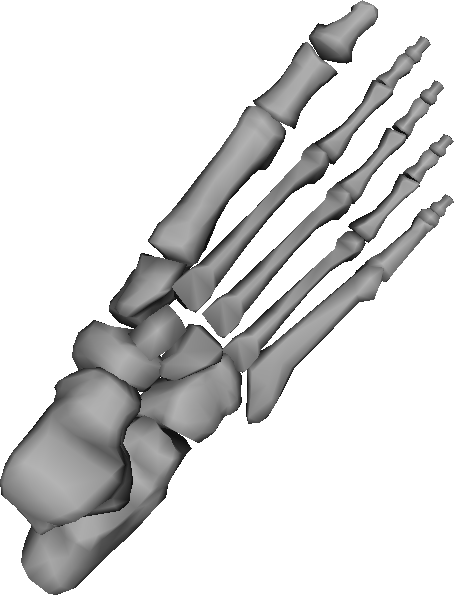
\includegraphics[width=0.45\textwidth]{pictures/image01.png}
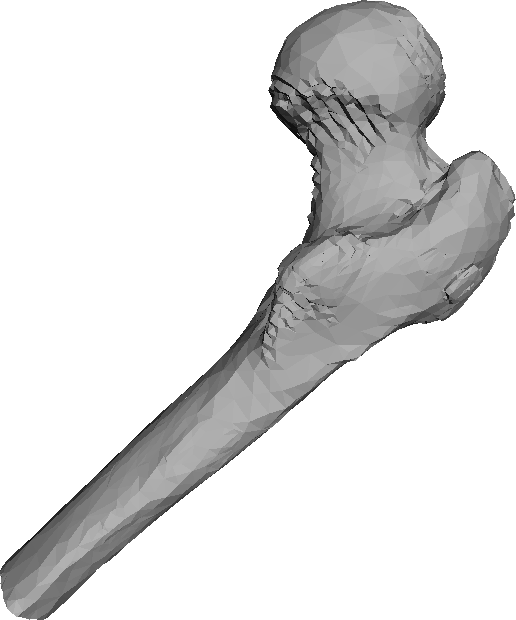
\includegraphics[width=0.45\textwidth]{pictures/image02.png}
\caption{Meshes generated from medical data. Data obtained from the AIM$@$SHAPE Shape Repository \cite{AIMSHAPE}}
\label{fig:example}
\end{figure}


This document is structured as follows. In Chapter~\ref{cha:Trabalhos relacionados} we present some previous work relevant to our problem. In Chapter~\ref{cha:Método proposto} we explain our proposal. In Chapter~\ref{cha:Resultados} we show our results. Finally, in Chapter~\ref{cha:Conclusão} we present our conclusion and future work.


 
  % -*- coding: utf-8; -*-

\chapter{Trabalhos relacionados}
\label{cha:Trabalhos relacionados}

Early smoothing methods tried to minimize... In the figure \ref{subfig:pictures/image01.png} we see...

\subimages{A set of three subfigures:
(a) describes the first subfigure;
(b) describes the second subfigure;
(c) describes the third subfigure.}{55}
{
 \subimage[Bamboo-pile Vertically Inserted Position]{.45}{pictures/image01.png}
 \subimage[Bamboo-pile Normal Inserted Position]{.45}{pictures/image02.png}\\
 \subimage[bamboo-pile Inserted 45° angle]{.45}{example-image}
}
\newpage
\csubimages{A set of six subfigures in two pages.}{55}
{
 \subimage[Bamboo-pile Vertically Inserted Position]{.45}{pictures/image01.png}
 \subimage[Bamboo-pile Normal Inserted Position]{.45}{pictures/image02.png}\\
 \subimage[bamboo-pile Inserted 45° angle]{.45}{example-image}
}
\ssubimages{A set of six subfigures in two pages.}{55}
{
 \subimage[Bamboo-pile Vertically Inserted Position]{.45}{pictures/image01.png}
 \subimage[Bamboo-pile Normal Inserted Position]{.45}{pictures/image02.png}\\
 \subimage[bamboo-pile Inserted 45° angle]{.45}{example-image}
}
  % -*- coding: utf-8; -*-
\chapter{Método proposto}
\label{cha:Método proposto}

Equation example 1:

\begin{equation}
\begin{split}
\min_u \int_{x_i\in X}\int_{x_j\in X} q_{ij} u_i u_j da da + \int_{x_i\in X}||x' - x_i|| u_i da \\
s.t. \ \ \ u\in[0,1] \ \ \land  \ \ \int_{x_i\in X}u da = a_0,
\end{split}
\end{equation}

Equation exmaple 2:

\begin{equation}
\begin{split}
\min_{\mathbf{u}} \alpha \mathbf{u}^T \mathbf{A}^T \mathbf{Q} \mathbf{A} \mathbf{u} +  \beta \mathbf{d}^T a' \mathbf{A} \mathbf{u} + \gamma \mathbf{u}^T \mathbf{G}^T \mathbf{G} \mathbf{u} + \delta\mathbf{f}^T a' \mathbf{A} \mathbf{u} \\
s.t. \ \ \ \mathbf{0} \leq \mathbf{u} \leq \mathbf{1} \land \mathbf{a}^T\mathbf{u}=a_0.
\end{split}
\end{equation}

Equation example 3:
\begin{align}
\mathbf{G}=(g_{ij}) = \left\lbrace
\begin{array}{ll}
\sum_{f_k\in N_f(f_i)} l_{ik} & i=j\\
-l_{ij} & e_{ij}\in E\\
0 & \text{otherwise}
\end{array}
\right.
\end{align}

\lstinputlisting[label=mean,title={Mean Filter},caption={Mean Filter},language=R]{codes/mean.R}

%% Algoritmo em portugues
\begin{algorithm}
\DontPrintSemicolon
\Entrada{Malha e quantidade de pontos a ser amostrado}
\Saida{Pontos amostrados na malha}
\BlankLine
\emph{Crie um vetor de números randômicos entre $[0,1]$ com a quantidade de pontos a ser amostrada e ordene-o}\;
\emph{Calcule a área total dos triângulos da malha}\;
\For{$i=0$ \KwTo numeroDePontos} {
  \emph{Navegue entre as faces acumulando a sua $\frac{area}{areaTotal}$ até achar a face com valor acumulado $\geqslant$ numerosRandomicos[i]}\;
  \emph{Pegue um ponto randômico dentro da face utilizando o método de Turk e adicione no vetor do resultado}\;
}
\caption{Escolha das amostras inicias}\label{alg:sampling}
\end{algorithm}\DecMargin{1em}

%% Algoritmo em ingles
%\begin{algorithm}
%\DontPrintSemicolon
%\KwIn{Malha e quantidade de pontos a ser amostrado}
%\KwOut{Pontos amostrados na malha}
%\BlankLine
%\emph{Crie um vetor de números randômicos entre $[0,1]$ com a quantidade de pontos a ser amostrada e ordene-o}\;
%\emph{Calcule a área total dos triângulos da malha}\;
%\For{$i=0$ \KwTo numeroDePontos} {
%  \emph{Navegue entre as faces acumulando a sua $\frac{area}{areaTotal}$ até achar a face com valor acumulado $\geqslant$ numerosRandomicos[i]}\;
%  \emph{Pegue um ponto randômico dentro da face utilizando o método de Turk e adicione no vetor do resultado}\;
%}
%\caption{Escolha das amostras inicias}\label{alg:sampling}
%\end{algorithm}\DecMargin{1em}







  % -*- coding: utf-8; -*-

\chapter{Resultados}
\label{cha:Resultados}

Table example. Table~\ref{tab:res} shows results. 

\begin{table}[!h]
\caption{Results for devil mesh}
\tiny
\begin{center}
\begin{tabular}{ m{1.1cm} m{0.95cm} m{0.95cm} m{0.95cm} m{0.95cm} m{0.95cm} m{0.95cm} m{0.95cm} m{0.95cm} m{0.95cm} } 
 & Mean Vertex Distance & L2 Vertex Based & Mean Quadric & MSAE & L2 Normal Based & Tangential & Mean Discrete Curvature & Area Error & Volume Error\\ 
 \hline 
\cite{FDC03} & 0.061277 & 0.110973 & 0.236219 & 19.697900 & 0.055170 & 0.047678 & 0.090284 & 0.051443 & 0.045645 \\ 
 \cite{JDD03} & 0.001293 & 0.002800 & 0.002289 & 21.237300 & 0.021589 & 0.013026 & 0.087991 & 0.000364 & 0.002621 \\ 
 \cite{SRML07} & 0.001439 & 0.002880 & 0.003540 & 14.043200 & 0.012654 & 0.008911 & 0.055849 & 0.007806 & 0.000582 \\ 
 \cite{ZFAT11} & \cellcolor{blue!25}0.000713 & \cellcolor{blue!25}0.001537 & 0.001824 & 12.171400 & \cellcolor{blue!25}0.009654 & \cellcolor{blue!25}0.005781 & \cellcolor{blue!25}0.054567 & 0.005617 & \cellcolor{blue!25}0.000425 \\ 
 \cite{HS13} & 0.002531 & 0.004560 & 0.007108 & 13.830100 & 0.017459 & 0.010314 & 0.114528 & 0.001686 & 0.001786 \\ 
 \cite{ZDZBL15} & 0.001623 & 0.003079 & 0.005048 & \cellcolor{blue!25}10.454200 & 0.015233 & 0.008054 & 0.094668 & 0.002629 & 0.001326 \\ 
 \cite{YRP16} & 0.000737 & 0.001548 & \cellcolor{blue!25}0.001493 & 16.880800 & 0.014129 & 0.006974 & 0.079952 & \cellcolor{blue!25}0.000209 & 0.002375 \\ 
 Ours & 0.000987 & 0.001902 & 0.002686 & 11.574200 & 0.010632 & 0.006796 & 0.075106 & 0.003970 & 0.000722 \\ 
 \end{tabular}
\end{center}
 \label{tab:res}
\end{table}

\section{Resultados comparativos}
  \chapter{Conclusão e trabalhos futuros}
\label{cha:Conclusão}

We proposed an algorithm for triangular mesh denoising with detail preservation...

\lstinputlisting[label=mean2,title={Mean Filter},caption={Mean Filter},language=R]{codes/mean.R}
  %% ...
  \arial
  \bibliographystyle{abnt-alf} % \bibliographystyle{abnt-num}
  \bibliography{main}
\end{document}
